% Options for packages loaded elsewhere
\PassOptionsToPackage{unicode}{hyperref}
\PassOptionsToPackage{hyphens}{url}
\PassOptionsToPackage{dvipsnames,svgnames*,x11names*}{xcolor}
%
\documentclass[
]{article}
\usepackage{lmodern}
\usepackage{amssymb,amsmath}
\usepackage{ifxetex,ifluatex}
\ifnum 0\ifxetex 1\fi\ifluatex 1\fi=0 % if pdftex
  \usepackage[T1]{fontenc}
  \usepackage[utf8]{inputenc}
  \usepackage{textcomp} % provide euro and other symbols
\else % if luatex or xetex
  \usepackage{unicode-math}
  \defaultfontfeatures{Scale=MatchLowercase}
  \defaultfontfeatures[\rmfamily]{Ligatures=TeX,Scale=1}
\fi
% Use upquote if available, for straight quotes in verbatim environments
\IfFileExists{upquote.sty}{\usepackage{upquote}}{}
\IfFileExists{microtype.sty}{% use microtype if available
  \usepackage[]{microtype}
  \UseMicrotypeSet[protrusion]{basicmath} % disable protrusion for tt fonts
}{}
\makeatletter
\@ifundefined{KOMAClassName}{% if non-KOMA class
  \IfFileExists{parskip.sty}{%
    \usepackage{parskip}
  }{% else
    \setlength{\parindent}{0pt}
    \setlength{\parskip}{6pt plus 2pt minus 1pt}}
}{% if KOMA class
  \KOMAoptions{parskip=half}}
\makeatother
\usepackage{xcolor}
\IfFileExists{xurl.sty}{\usepackage{xurl}}{} % add URL line breaks if available
\IfFileExists{bookmark.sty}{\usepackage{bookmark}}{\usepackage{hyperref}}
\hypersetup{
  colorlinks=true,
  linkcolor=red,
  filecolor=Maroon,
  citecolor=Blue,
  urlcolor=Blue,
  pdfcreator={LaTeX via pandoc}}
\urlstyle{same} % disable monospaced font for URLs
\usepackage[margin=1in]{geometry}
\usepackage{graphicx}
\makeatletter
\def\maxwidth{\ifdim\Gin@nat@width>\linewidth\linewidth\else\Gin@nat@width\fi}
\def\maxheight{\ifdim\Gin@nat@height>\textheight\textheight\else\Gin@nat@height\fi}
\makeatother
% Scale images if necessary, so that they will not overflow the page
% margins by default, and it is still possible to overwrite the defaults
% using explicit options in \includegraphics[width, height, ...]{}
\setkeys{Gin}{width=\maxwidth,height=\maxheight,keepaspectratio}
% Set default figure placement to htbp
\makeatletter
\def\fps@figure{htbp}
\makeatother
\setlength{\emergencystretch}{3em} % prevent overfull lines
\providecommand{\tightlist}{%
  \setlength{\itemsep}{0pt}\setlength{\parskip}{0pt}}
\setcounter{secnumdepth}{-\maxdimen} % remove section numbering
\usepackage{pdfpages}
\usepackage{amsmath}
\usepackage{booktabs}
\usepackage{longtable}
\usepackage{array}
\usepackage{multirow}
\usepackage{wrapfig}
\usepackage{float}
\usepackage{colortbl}
\usepackage{pdflscape}
\usepackage{tabu}
\usepackage{threeparttable}
\usepackage{threeparttablex}
\usepackage[normalem]{ulem}
\usepackage{makecell}
\usepackage{xcolor}
\newlength{\cslhangindent}
\setlength{\cslhangindent}{1.5em}
\newenvironment{cslreferences}%
  {}%
  {\par}

\author{}
\date{\vspace{-2.5em}}

\begin{document}

\pagenumbering{gobble}

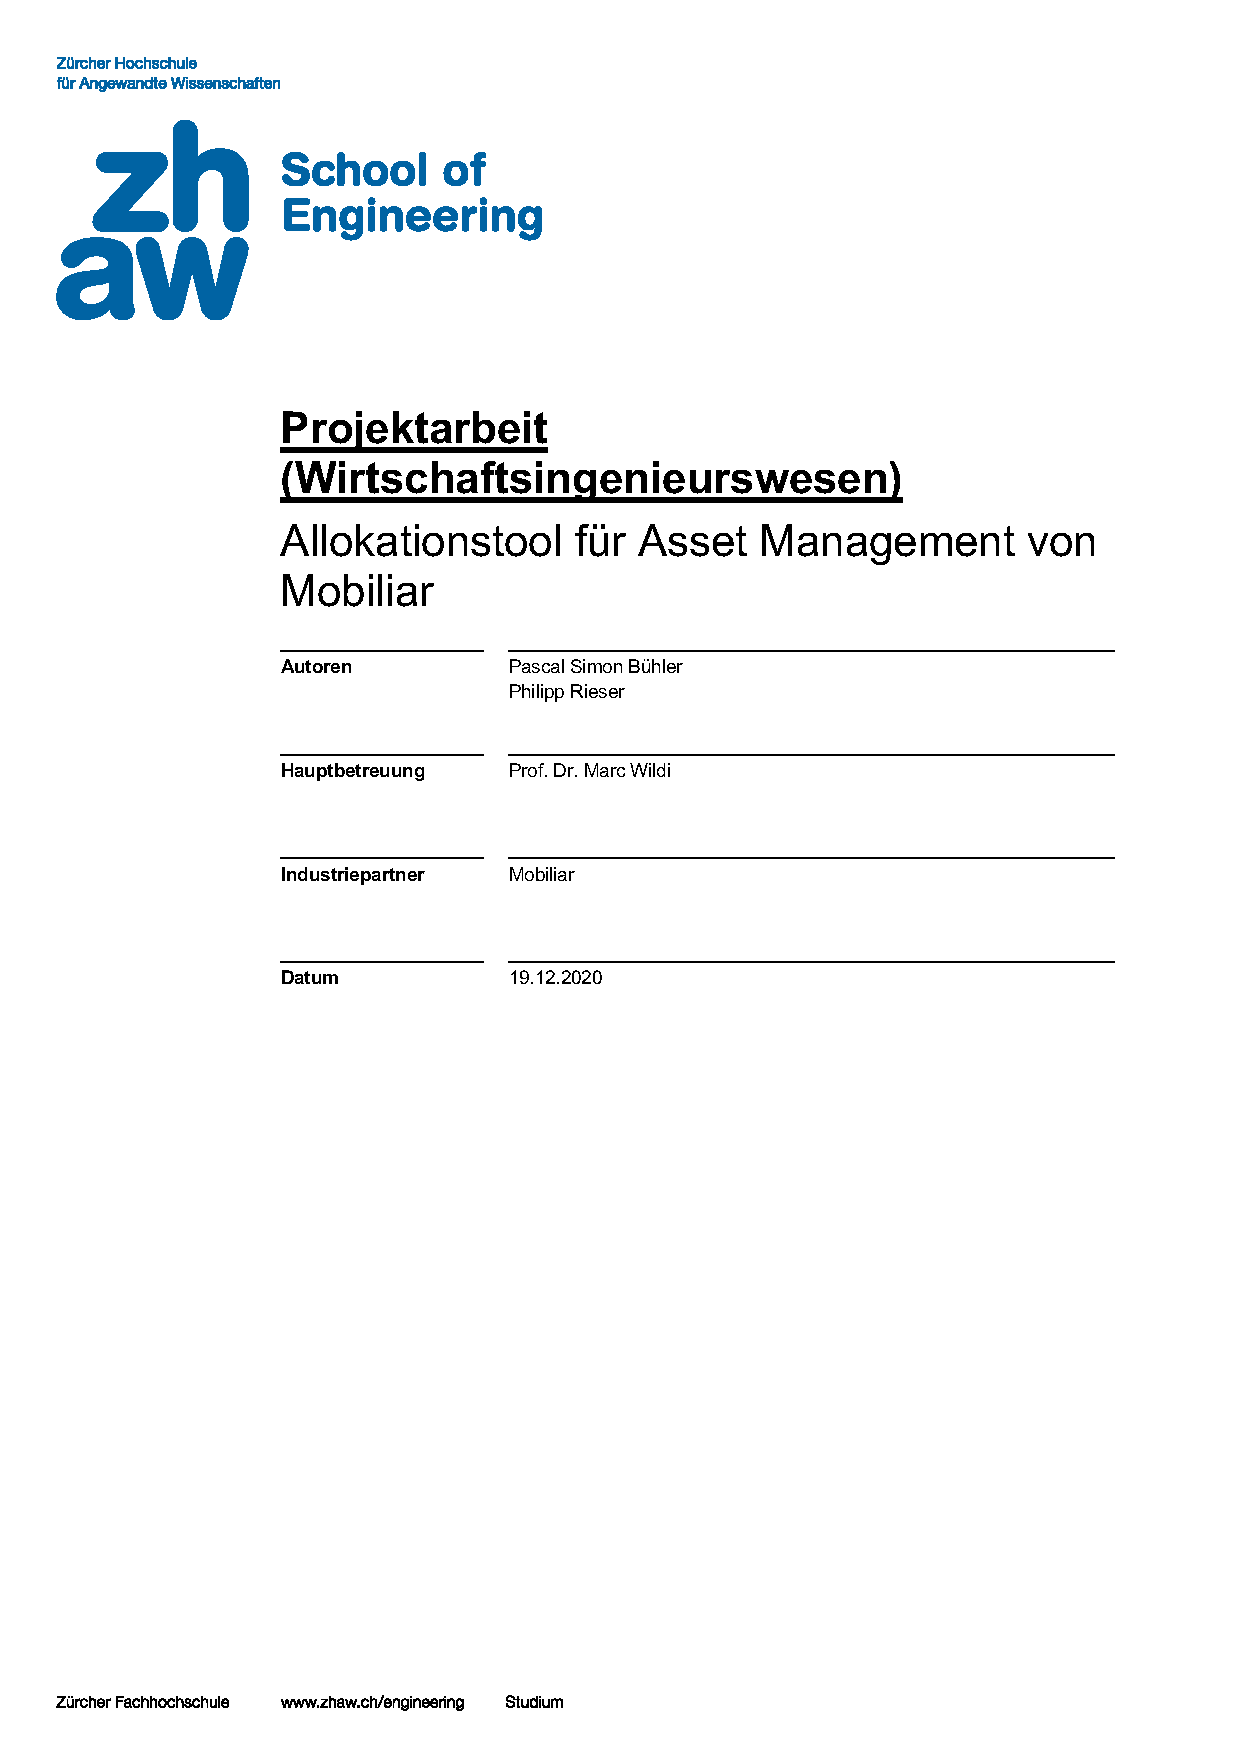
\includepdf{add/titelblatt.pdf}
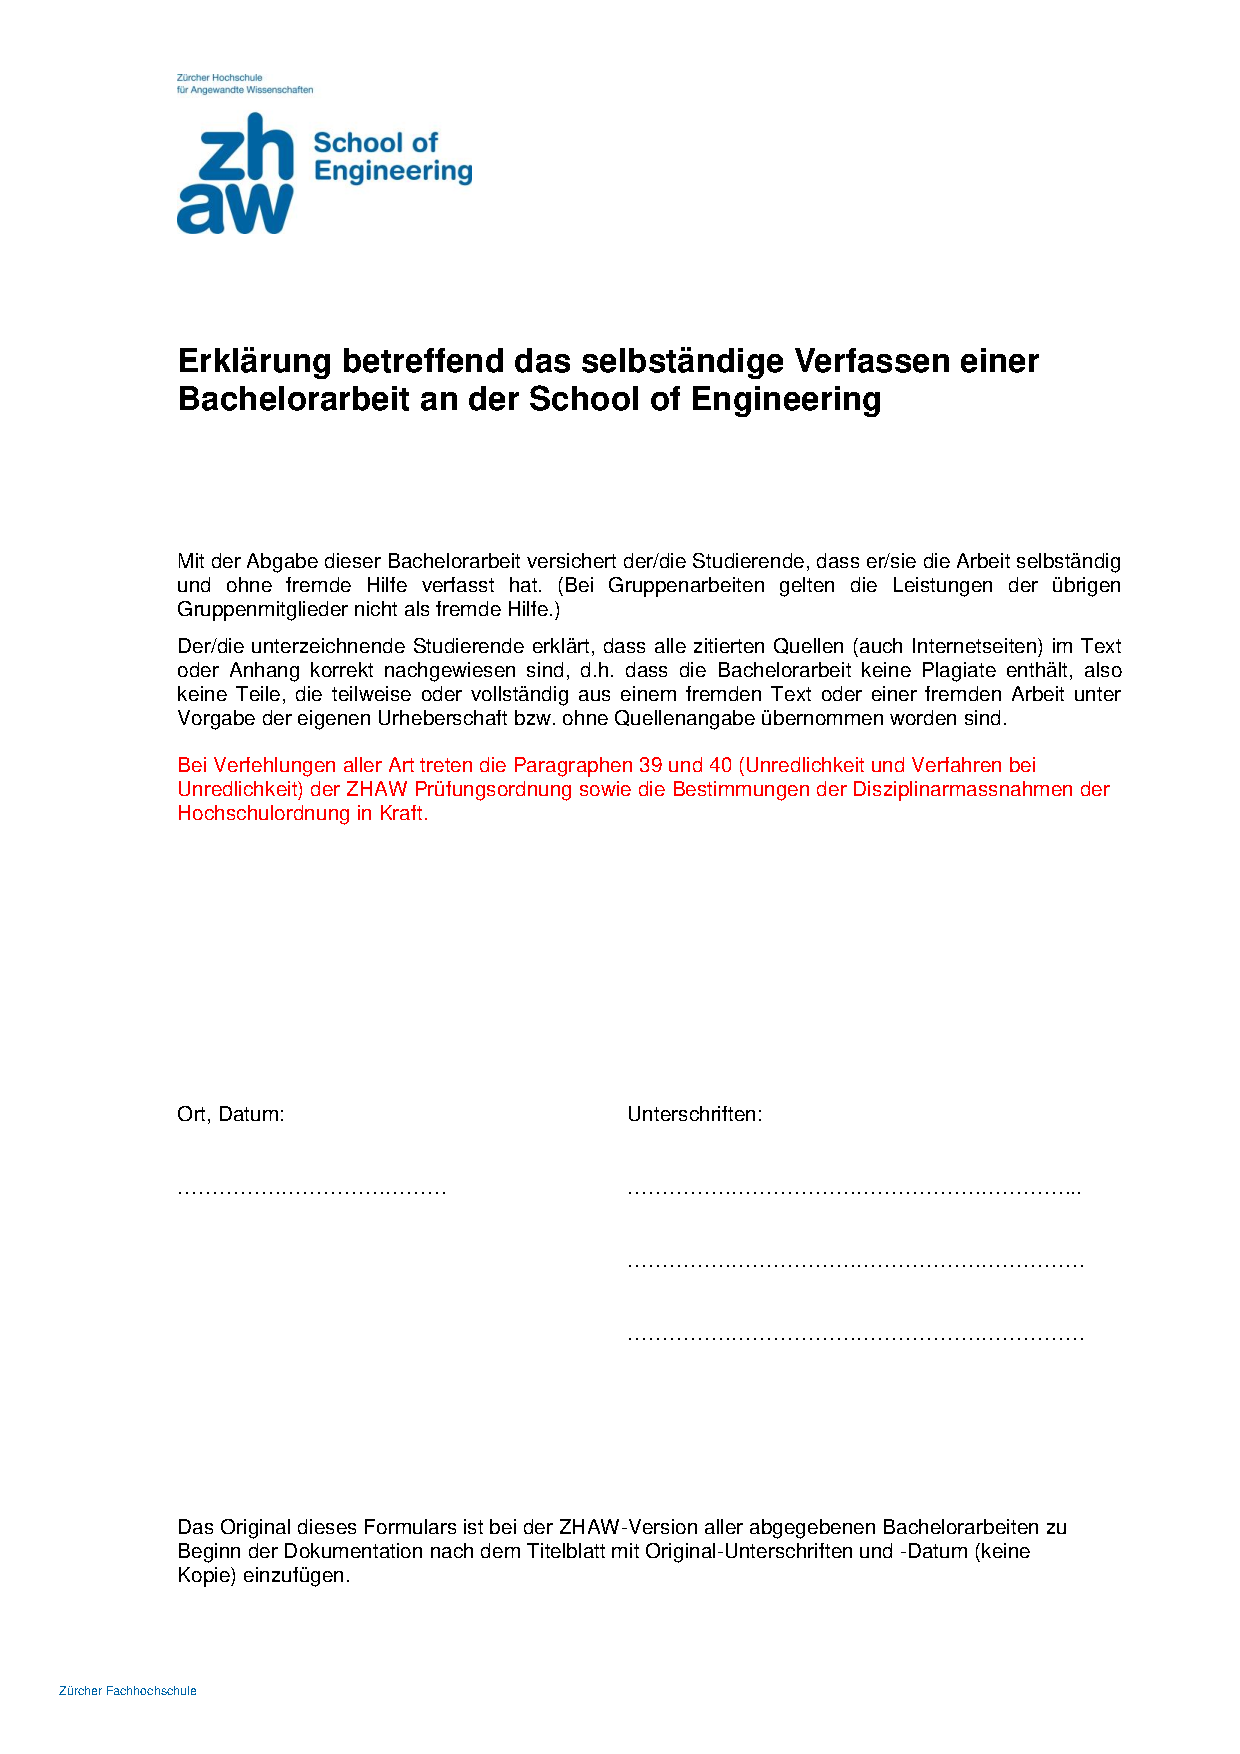
\includepdf{add/Erklaerung_BA.pdf}

\tableofcontents

\newpage

\hypertarget{abstract}{%
\subsection{Abstract}\label{abstract}}

\newpage

\pagenumbering{arabic}

\hypertarget{introduction}{%
\subsection{1. Introduction}\label{introduction}}

The main purpose of trading is buying and selling stocks, bonds, or
other financial instruments with increasing the returns of the
investments in mind while maintaining relatively low risk. With the help
of a trading strategy, an investor can try to improve his performance.
One can simply divide the strategies into passive and active. The
praised and well established passive strategy buy-and-hold takes no
short price movements into account. Positioning and trading based on
these short price movements are considered active trading.

This paper applies time-series analysis to these short price movements
to create active trading strategies. The objective of these developed
strategies is to outperform the buy-and-hold strategy.

\hypertarget{the-data-used-in-this-paper}{%
\subsubsection{1.1. The data used in this
paper}\label{the-data-used-in-this-paper}}

The dataset which will be analyzed in this paper contains 4 tradeable
indexes, a visualization of the data is shown below in figure
\ref{fig:chap1.1}.

\begin{figure}

{\centering 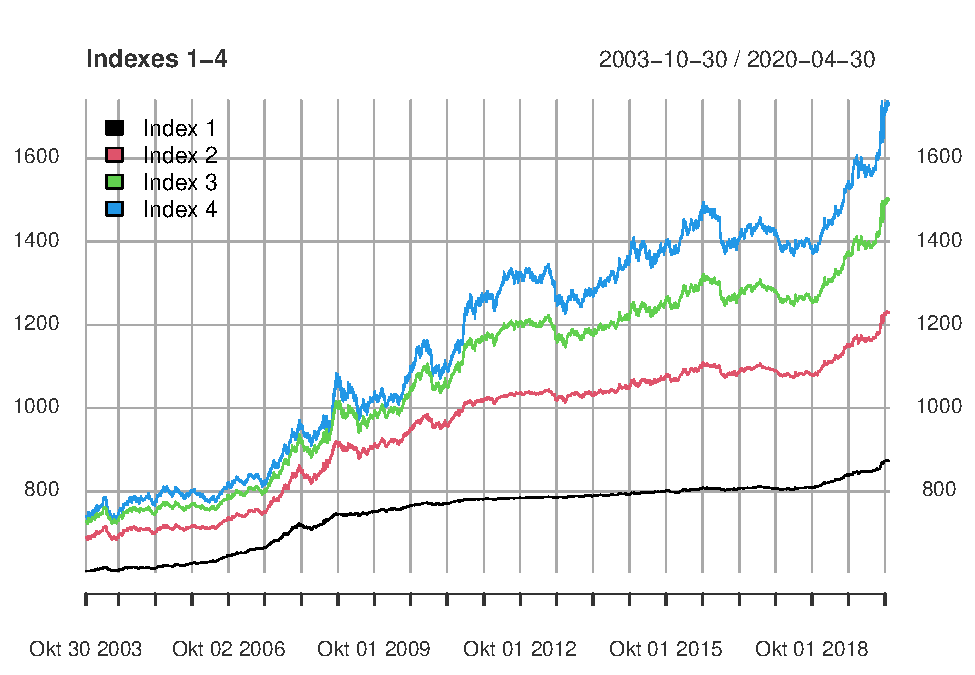
\includegraphics[width=0.7\linewidth]{00_main_files/figure-latex/chap1.1-1} 

}

\caption{Visualization of the 4 indexes}\label{fig:chap1.1}
\end{figure}

Each time-series has 4306 observations and starts from October 2003 to
April 2020. In all indexes is an upward drift observable, during the
time period of the great recession (2008) is a slight bump visible. Also
later in 2013 and 2016 are small break-ins evident. More interesting is
the up and down behavior at the end of the series during the Covid19
pandemic.

\newpage

In addition, to the indexes, the dataset contains 8 different interest
rates of treasury bonds which will be used for further analysis. A few
key-values of the interest rates are shown in the following table
\ref{tab:inttable}.

\begin{table}[!h]

\caption{\label{tab:inttable}Summary of the 8 interest rates.}
\centering
\begin{tabular}[t]{llrrrr}
\toprule
  & Maturity & Mean & Volatility & Min. & Max.\\
\midrule
\cellcolor{gray!6}{Interest 1} & \cellcolor{gray!6}{3M} & \cellcolor{gray!6}{4.09} & \cellcolor{gray!6}{4.95} & \cellcolor{gray!6}{-0.28} & \cellcolor{gray!6}{16.27}\\
Interest 2 & 6M & 4.47 & 5.05 & 0.01 & 16.73\\
\cellcolor{gray!6}{Interest 3} & \cellcolor{gray!6}{1Y} & \cellcolor{gray!6}{4.64} & \cellcolor{gray!6}{4.22} & \cellcolor{gray!6}{0.20} & \cellcolor{gray!6}{10.51}\\
Interest 4 & 2Y & 5.42 & 4.58 & 0.49 & 16.58\\
\cellcolor{gray!6}{Interest 5} & \cellcolor{gray!6}{3Y} & \cellcolor{gray!6}{6.16} & \cellcolor{gray!6}{4.33} & \cellcolor{gray!6}{0.75} & \cellcolor{gray!6}{16.51}\\
\addlinespace
Interest 6 & 5Y & 7.41 & 3.82 & 1.06 & 16.44\\
\cellcolor{gray!6}{Interest 7} & \cellcolor{gray!6}{7Y} & \cellcolor{gray!6}{9.50} & \cellcolor{gray!6}{3.31} & \cellcolor{gray!6}{1.71} & \cellcolor{gray!6}{16.63}\\
Interest 8 & 10Y & 11.61 & 2.93 & 3.13 & 17.47\\
\bottomrule
\end{tabular}
\end{table}

A typical characteristic of interest rates is shown in the given data. A
bond with longer maturities is often associated with higher returns
compared with those with shorter maturities. An investor which invests
in short-term treasury bonds will have his gain earlier but will be
confronted with a lower return.

A more in depth analysis of the given dataset will follow in section
\protect\hyperlink{ts-analysis}{3.1}.

\hypertarget{ojective-of-this-paper}{%
\subsubsection{1.2. Ojective of this
paper}\label{ojective-of-this-paper}}

The objective of this paper is to trade these 4 indexes with an active
trading strategy. The main objective is to outperform the passive
buy-and-hold strategy. Methods such as the Moving-Average-Filter or the
ARMA-GARCH-Model provide signals for either long or short the position
to maximize the return of the investments in these indexes.

The performance of these strategies are build open various different
parameters and conditions. The lengths of the filters applied to a
Moving-Average may result in different solutions. Models could perform
differently for any given length of the in-sample or out-of-sample
scope. The necessity of including a historical crisis in the
starting-sample can decide if a model performs better or worse than
another. The correct validation of model parameters could have a
significant impact on the forecasts.

In addition to all criteria and conditions, the strategies can be
further adjusted by composing different weighted portfolios. Estimated
predicted volatility can be used to modulate the position size to
mitigate the risk.

Challenging will be finding the most optimal model in this wide field of
conditions and parameters. The buy-and-hold strategy will be used as a
benchmark to be compared with the developed active trading strategies.
Computing and comparing the Sharpe ratios of each model can serve as an
indicator to rely on for better or worse models.

\newpage

\hypertarget{theory}{%
\subsection{2. Theory}\label{theory}}

It is assumed that the reader of this paper already has basic knowledge
of the mathematical principles of time series analysis. Therefore, this
section will only briefly describe the mathematical models and
processes.

\hypertarget{time-series}{%
\subsubsection{2.1. Time-Series}\label{time-series}}

Almost anything with a data point to a given timestamp can be named a
time-series. The monthly gross domestic product, the weekly US gasoline
production, or daily stock price movements. In this paper lies the focus
of the analysis of financial time series. Due to trades often only take
place during the week, there are gaps in the time series on the
weekends, an exception would be the trading of cryptocurrencies like
Bitcoin which are also tradeable at the weekends.

A series of data points with more or less equidistant time points \(t\)
with the sample length of \(T\), is called a time-series
\(x_{t}, t=1,...,T\) {[}1{]}. The analysis of a time-series \(x_{t}\)
involves creating a reasonable model that can be utilized to perform
forecast predictions.

\hypertarget{stationarity}{%
\paragraph{2.1.1. Stationarity}\label{stationarity}}

~

In order to fit a suitable model with a given time series \(x_{t}\), the
assumptions of stationarity must be met. In this practical application,
only the following weak-stationarity properties are required.

\begin{equation}
  \label{eq:mean}
  E[x_{t}]=\mu
\end{equation}

\begin{equation}
  \label{eq:var}
  Var(x_{t})=\sigma_{x}^{2}
\end{equation}

\begin{equation}
  \label{eq:cov}
  Cov(x_{t}, x_{t-k})=R(k)
\end{equation}

Many financial time-series are subject to shift, trends or changing
volatility. In figure \ref{fig:chap2.1} are the stock prices of Alphabet
Inc Class A (Google) visualized. This time-series shows a clear upwards
drift and towards the end the volatility increases.

\begin{figure}

{\centering 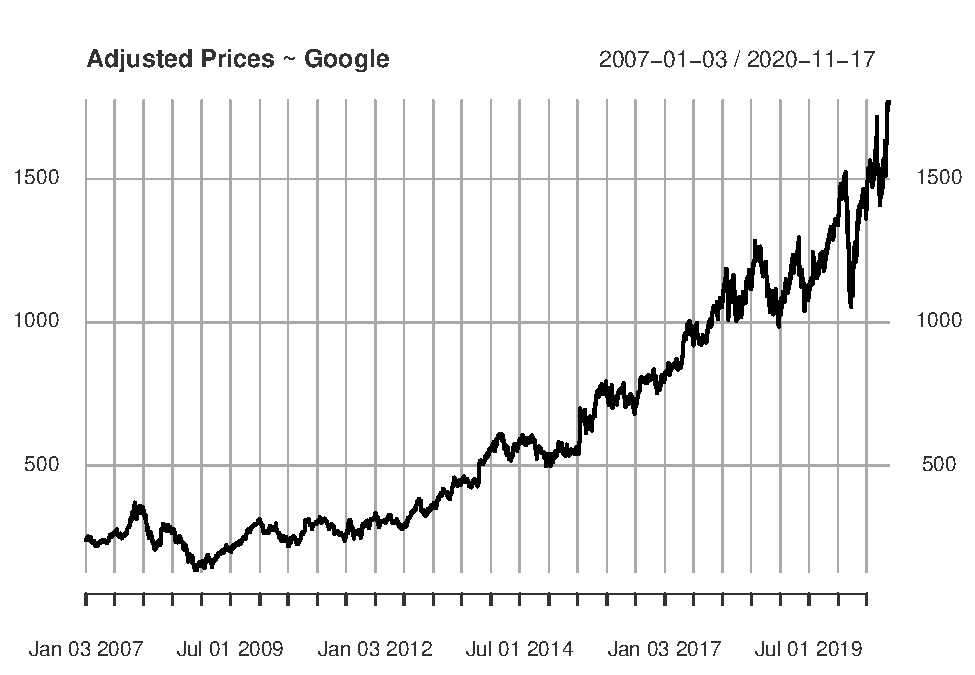
\includegraphics[width=0.7\linewidth]{00_main_files/figure-latex/chap2.1-1} 

}

\caption{Visualization of the adjusted prices of the Alphabet Inc Class A Stock.}\label{fig:chap2.1}
\end{figure}
\newpage

To improve the violated properties the first difference can be applied
and additionally a logarithmic transformation can be performed {[}2{]}.
The log-returns transformation can only performed to strict positive
data.

\[\mathrm{LogReturn} = \mathrm{log}(x_{t})-\mathrm{log}(x_{t-1})\]

The result is the so-called log-returns.

\begin{figure}

{\centering 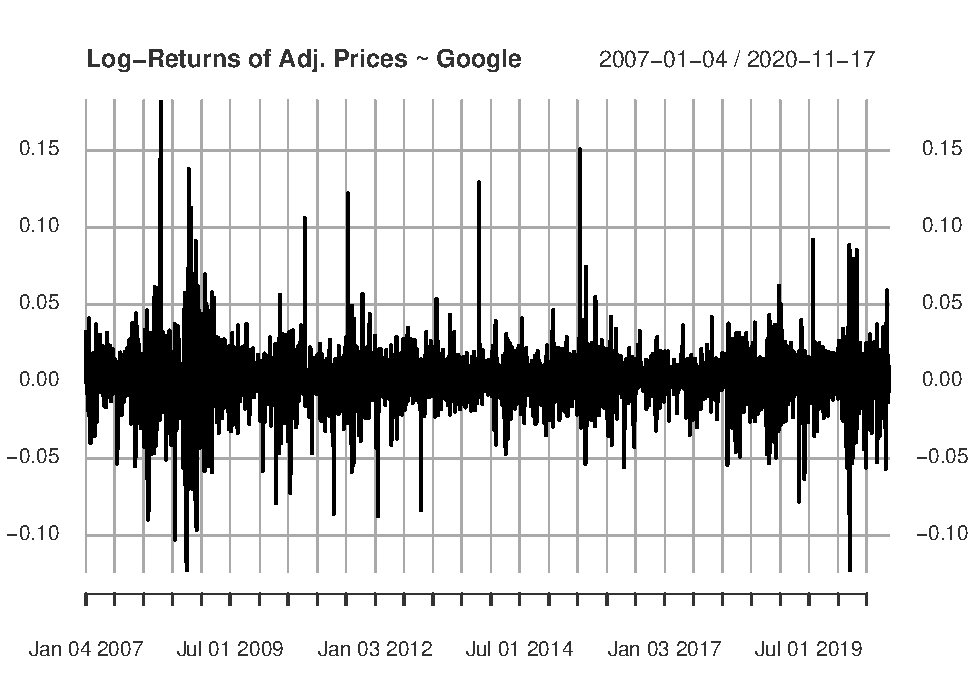
\includegraphics[width=0.7\linewidth]{00_main_files/figure-latex/chap2.2-1} 

}

\caption{Visualization of the Log-Returns}\label{fig:chap2.2}
\end{figure}

Applying the transformation to the data causes the drift to disappear,
but the series still contains stronger and weaker volatile phases. This
effect often occurs in non-stationary financial data and is called
volatility cluster. This special property is used for the modelling of
forecast models, which will be discussed in chapter
\protect\hyperlink{models-section}{2.2}.

\hypertarget{autocorrelation}{%
\paragraph{2.1.2. Autocorrelation}\label{autocorrelation}}

~

The autocorrelation function (ACF) reveals how the correlation between
any two data points of the time series changes as their separation
changes {[}3{]}. More precisely, acf measures the dependence between
\(x_{t}\) and \(x_{t \pm k}\) at lag \(k\). The partial autocorrelation
(PACF) measures the dependency between \(x_{t}\) and \(x_{t-k}\) at lag
\(k\) {[}1{]}. For stationary time series, ACF can be used to identify
the model order of a MA-process, PACF for AR-processes.

In the following figure \ref{fig:chap2.1.2} are ACF and PACF of the
non-stationary adjusted Google stock visualized. Both graphics show the
typical pattern of a non-stationary time series. The plot above shows
the dependence structure of the time series. This means that it takes a
long time until the series changes. Often a large value is followed by
another large value, which indicates a strong trend. This property of
the series can be seen in figure \ref{fig:chap2.1} as the long upward
drift. The plot below indicates a significant partial autocorrelation at
lag \(k=1\).

In the following section \protect\hyperlink{models-section}{2.2.} the
characteristics of the autocorrelation function can be used for the
verification of ARIMA and ARCH-processes.

\begin{figure}

{\centering 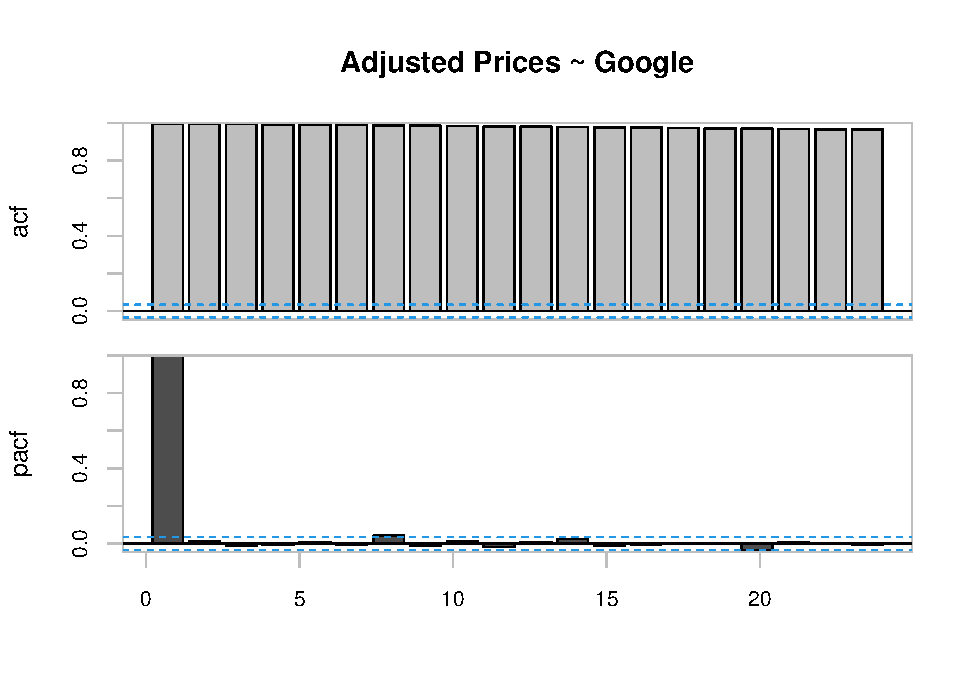
\includegraphics[width=0.7\linewidth]{00_main_files/figure-latex/chap2.1.2-1} 

}

\caption{Acf and Pacf of the Adjusted Prizes of Google.}\label{fig:chap2.1.2}
\end{figure}

\newpage

\hypertarget{models-section}{%
\subsubsection{2.2. Models}\label{models-section}}

The following processes are used to determine certain properties and
characteristics of a time series so that they are transformed into a
model. The goal is to fit the time series as well as possible in order
to create reliable forecasts.

\hypertarget{arima}{%
\paragraph{2.2.1. ARIMA}\label{arima}}

~

An ARIMA(\emph{p},\emph{d},\emph{q}) process is defined as follows.

\begin{equation} \label{eq:arima}
  x_{t}=c+a_{1}x_{t-1}+...+a_{p}x_{t-p}+\epsilon_{t}+b_{1}\epsilon_{t-1}+...+b_{q}\epsilon_{t-q}
\end{equation}

\begin{itemize}
\tightlist
\item
  \(p\) and \(q\) are the AR- and MA-model orders
\item
  \(a\) and \(b\) are the AR- and MA-model parameters
\item
  \(d\) is the differential parameter
\item
  \(\epsilon_t\) is a white noise sequence
\item
  \(x_t\) is the given data \(x_{1},...,x_{T}\)
\end{itemize}

The mean of an ARIMA-process can be computed as:

\[\mu=\frac{c}{1-a_{1}-...-a_{p}}\]

ARIMA processes can be divided into 4 different models. Choosing a model
that best represents the time series is a difficult task. The goal is to
find the best possible model with as few parameters as possible.

The previously introduced ACF and PACF can help to determine the orders
of simple models. Provided that the time series is stationary, the model
orders can be determined directly. For an AR(\emph{p})-process
(ARIMA(\emph{p},\emph{0},\emph{0})), the ACF plot will gradually
decrease and simultaneously the PACF should have a sharp drop after
\emph{p} significant lags. For an MA(\emph{q})-process
(ARIMA(\emph{0},\emph{0}.\emph{q})) the opposite is true, the ACF should
show a sharp drop after a certain \emph{q} number of lags while PACF
should show a gradual decreasing trend. If both ACF and PACF show a
gradual decreasing pattern, then the
ARIMA(\emph{p},\emph{0},\emph{q})-process should be considered for
modeling {[}4{]}. If the time series is not stationary, differentiation
can be considered (ARIMA(\emph{p},\emph{d},\emph{q})).

\newpage

The application of an analysis method to Google prices finds an
ARIMA(\emph{1},\emph{1},\emph{0}) as the optimal model. This makes sense
if you look back at figure \ref{fig:chap2.1.2}. Long dependency
structures in the ACF plot indicating an AR(\emph{p}) process and at the
same time after lag=\(1\)=\emph{p} the PACF has a strong drop. The
differential operator \emph{d}=\(1\) transforms the non-stationary
series into a stationary one.

\begin{figure}

{\centering 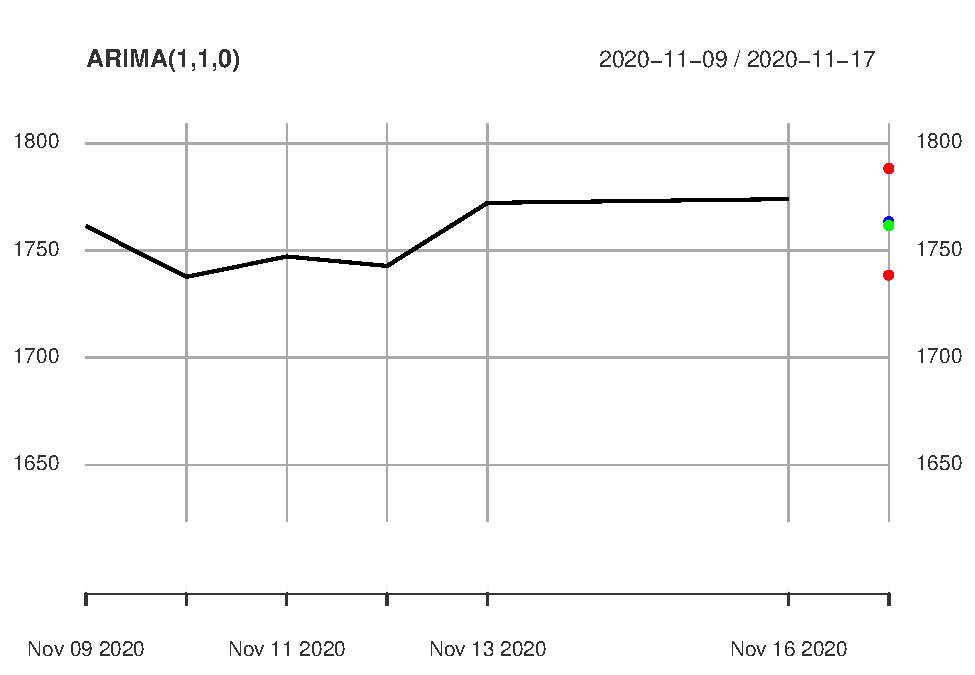
\includegraphics[width=0.7\linewidth]{00_main_files/figure-latex/chap2.2.1-1} 

}

\caption{ARIMA-Forecast}\label{fig:chap2.2.1}
\end{figure}

\hypertarget{arch-garch-section}{%
\paragraph{2.2.2. ARCH \& GARCH}\label{arch-garch-section}}

~

The volatility clustering mentioned in section
\protect\hyperlink{stationarity}{2.1.1} can be handled with an
auto-regressive conditional heteroscedastic process.

\begin{align} \label{eq:arch}
  \epsilon_{t} &= \mathrm{log}(x_{t})-\mathrm{log}(x_{t-1}) \nonumber \\
  \epsilon_{t} &= \sigma_{t}u_{t} \\
  \sigma_{t}^{2} &=c \sigma^{2}+\sum_{k=1}^{m}\beta_{k}\epsilon_{t-k}^{2} \nonumber
\end{align}

with:

\begin{itemize}
\tightlist
\item
  \(x_{t}\) is the original data (often non-stationary)
\item
  \(\epsilon_{t}\) is the stationary log-return
\item
  \(u_{t}\) is independent and identically distributed (iid) and
  standardized random variable
\item
  \(\sigma^{2}\) is the unconditional variance of the process
  \(\epsilon_{t}\).
\item
  \(\sigma_{t}^{2}\) is the conditional variance of the process
  \(\epsilon_{t}\).
\end{itemize}

The ARCH-process can be generalized by adding the lagged conditional
variances to the equation \ref{eq:arch}.

\begin{align} \label{eq:garch}
  \epsilon_{t} &= \mathrm{log}(x_{t})-\mathrm{log}(x_{t-1}) \nonumber \\
  \epsilon_{t} &= \sigma_{t}u_{t} \\
  \sigma_{t}^{2} &=c \sigma^{2}+\sum_{j=1}^{n}\alpha_{j}\sigma_{t-j}^{2}+\sum_{k=1}^{m}\beta_{k}\epsilon_{t-k}^{2} \nonumber
\end{align}

\hypertarget{arima-garch}{%
\paragraph{2.2.3. ARIMA-GARCH}\label{arima-garch}}

~

Another process is the combination of ARIMA and GARCH processes.

\begin{eqnarray}
y_{t}&=&\mu + a_{1}y_{t-1}+...+a_{p}y_{t-p}+\epsilon_{t}+b_{1}\epsilon_{t-1}+...+b_{q}\epsilon_{t-q} \label{eq:arima-garch1} \\
\epsilon_{t}&=&\sigma_{t}u_{t} \nonumber \\
\sigma_{t}^{2}&=&c\sigma^{2}+\sum_{j=1}^{n}\alpha_{j}\sigma_{t-j}^{2}+\sum_{k=1}^{m}\beta_{k}\epsilon_{t-k}^{2} \label{eq:arima-garch2}
\end{eqnarray}

Is called the mean-equation \ref{eq:arima-garch1}

Is called the variance-equation \ref{eq:arima-garch2}

{[}5{]}

\newpage

\hypertarget{moving-average-filters}{%
\subsubsection{2.3. Moving Average
Filters}\label{moving-average-filters}}

moving average filters are basically used to identify trends and smooth
out price fluctuations. As a commonly used tool moving average filters
are very simple in its usage, historical data was summarized and divided
bi the length of the filter. The actual challenge in using Moving
average filters is to figure out which length of the filter brings the
most useful information.

\hypertarget{equally-weighted-moving-average}{%
\paragraph{2.3.1. Equally-weighted Moving
Average}\label{equally-weighted-moving-average}}

~

SMA stands for Simple Moving Average which. depending on the length of
the filter(l) l obervations since the last noted observation will be
considered. theyre getting summarized and divided by the filterlength
equals the EqMA. For every timestep a new observation is considered and
the last one eliminated.

EqMA

\begin{equation}
  \label{eq:eqma}
  y_{t}=\frac{1}{L}\sum_{k=0}^{L-1}x_{t-k}
\end{equation}

\begin{itemize}
\tightlist
\item
  \({L}\) = filterlength
\end{itemize}

\hypertarget{exponentially-weighted-moving-average}{%
\paragraph{2.3.2. Exponentially-weighted Moving
Average}\label{exponentially-weighted-moving-average}}

~

Since not all observations are having the same influence of future value
we can apply a weight to past observations. One method will be
exponentially weighted Moving average. So we chose an optimal parameter
to give past observations weights decreasing by alpha

A skillfull trader chose an optimal to increase the performace of the
measurement. Weights could also be given individually by adding a weight
vector to the filter.

EMA

\begin{equation}
  \label{eq:ema}
  y_{t}=\frac{1}{\sum_{k=0}^{m}\alpha^{k}}\sum_{k=0}^{m}\alpha^{k}x_{t-k}
\end{equation}

\begin{itemize}
\tightlist
\item
  \({m}\) = filterlength
\item
  \({\alpha}\) = Parameter to weigh the observations
\end{itemize}

\hypertarget{moving-average-crossings}{%
\paragraph{2.3.3. Moving Average
Crossings}\label{moving-average-crossings}}

~

\begin{equation}
  \label{eq:mac}
  y_{t}=\frac{1}{L_1}\sum_{k=0}^{L_1-1}x_{t-k} - \frac{1}{L_2}\sum_{k=0}^{L_2-1}x_{t-k}
\end{equation}

\begin{itemize}
\tightlist
\item
  \({L_1}\) = filterlength 1
\item
  \({L_2}\) = filterlength 2
\item
  \({0 < \alpha < 1}\) = Parameter to weigh the observations
\end{itemize}

Moving average crossings are basically just different MA's with
different lengths applied to a time-series. The points the filters then
cross will be used as a trading signal to go long, short or hold.

An easy example of Ma average crossings with 2 mas of different length
is visualized in \# \ref{fig:chap2.1}.

\begin{center}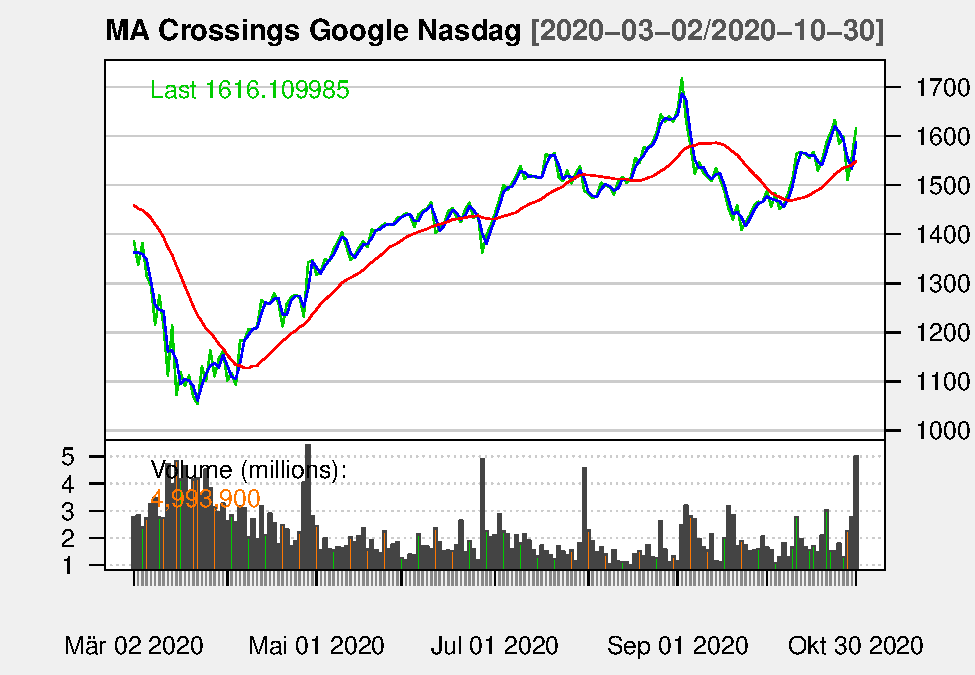
\includegraphics[width=0.7\linewidth]{00_main_files/figure-latex/chap2.3.3 -1} \end{center}

\newpage

\hypertarget{real-strength-index}{%
\subsubsection{2.4. Real Strength Index}\label{real-strength-index}}

\hypertarget{sharpe-ratio}{%
\subsubsection{2.5. Sharpe Ratio}\label{sharpe-ratio}}

~

Sharpe ratio is a very powerful and widely used ratio to measure
performance. It describes return per risk

\begin{equation}
  \label{eq:Sharperatio}
  \mathrm{SharpeRatio}=\frac{R_{p}-R_{f}}{\sigma}
\end{equation}

\begin{itemize}
\tightlist
\item
  \({R_p}\) = Return of Portfolio
\item
  \({R_p}\) = Risk free Rate, mostly treasury bonds
\item
  \({\sigma_p}\) = standard deviation of portfolios excess return (risk)
\end{itemize}

\hypertarget{carry}{%
\subsubsection{2.6. Carry}\label{carry}}

carry trades are trading strategies where usually money is borrowed at a
lower intrest rate than the investment is gioving in return. the risk of
this strategy is based in the currency risk.

\hypertarget{value}{%
\subsubsection{2.7. Value}\label{value}}

\hypertarget{bollinger-bands}{%
\subsubsection{2.8 Bollinger bands}\label{bollinger-bands}}

~

Bollinger bands are a analysis tool founded by John Bollinger. It
contains a moving average and an upper and lower band . The bands are
defined by adding a constant\({K}\) times a standard deviation
\({\sigma_t}\) to the \emph{Moving Average} for the upper , and
subtracting it for the lower band.

\begin{equation}
  \label{eq:lower and upper bollingerbands}
  \mathrm{U_t}=MA_{t}+K\sigma, L_{t}=MA_{t}-K\sigma
\end{equation}

the variance from bollingers theory is calculated by:

\begin{equation}
  \label{eq:variance bollingerbands}
  \mathrm{\sigma_{t}^2}=\frac{1}{N}\sum_{k=0}^{N-1}(x_{t-k} -MA_t)^2
\end{equation}

the calculated \({\sigma_t}\) could be problematic because its derived
from the original series and increases with the level. Therefore an
other method to calculate the standart deviation could be used.

\begin{itemize}
\tightlist
\item
  \({N}\) = usually the filterlength and the lentgh considered for
  \({\sigma}\) the same
\item
  \({K}\) = Constant usually equals 2
\item
  \(\sigma_p\) = standard deviation of the series
\item
  \({U_t}\) = upper band
\item
  \({L_t}\) = lower band
\end{itemize}

\begin{center}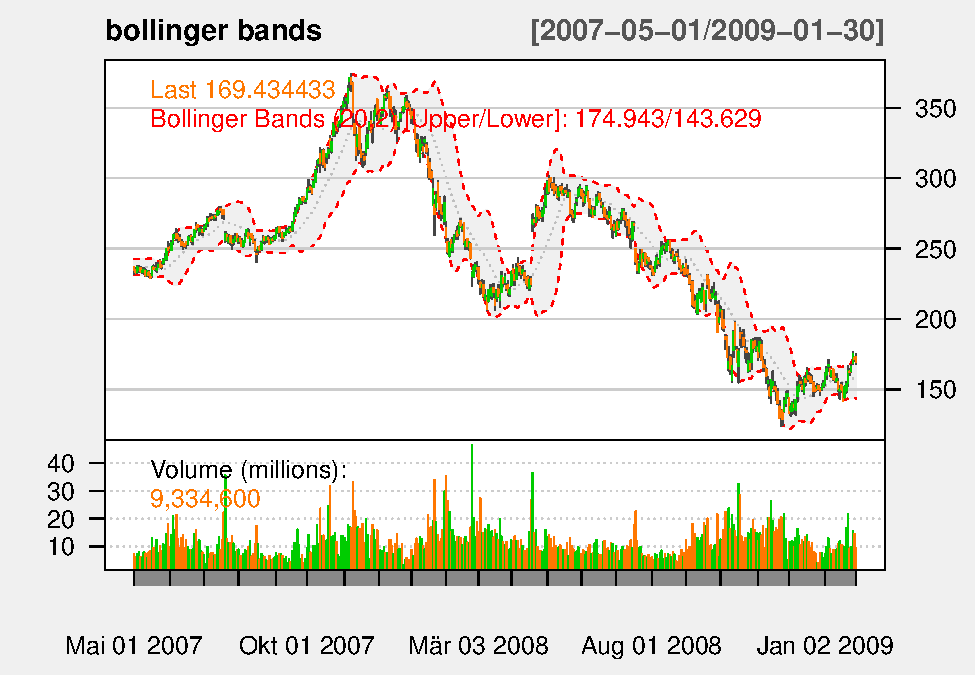
\includegraphics[width=0.7\linewidth]{00_main_files/figure-latex/chap2.8 -1} \end{center}

\newpage

\hypertarget{methodology}{%
\subsection{3. Methodology}\label{methodology}}

In this section models were created trying to outperform the buy and
hold strategy. starting with the usage of the simplest models , diffrent
aproaches were chosen to fullfill the goal.

\hypertarget{ts-analysis}{%
\subsubsection{3.1. Time-Series Analysis}\label{ts-analysis}}

Plots of the timeseries, decomposition. Stationarity (refer to the
theory section)

\hypertarget{using-simple-methods}{%
\subsubsection{3.2 using simple methods}\label{using-simple-methods}}

\begin{figure}

{\centering 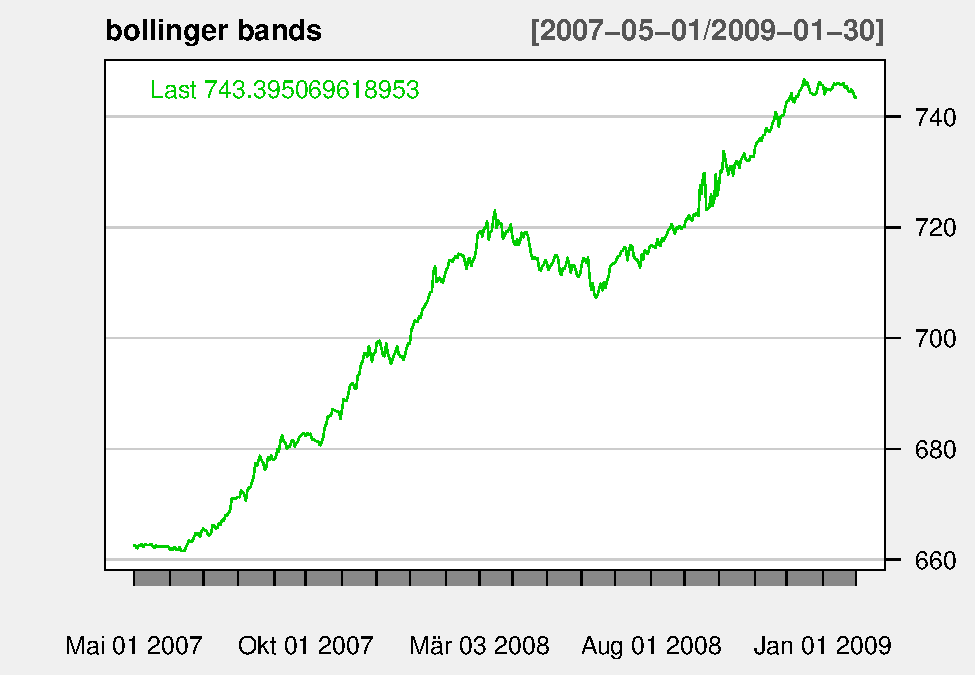
\includegraphics[width=0.7\linewidth]{00_main_files/figure-latex/chap3.2-1} 

}

\caption{conversion data}\label{fig:chap3.2}
\end{figure}

\newpage

\hypertarget{conclusion}{%
\subsection{4. Conclusion}\label{conclusion}}

\newpage

\hypertarget{references}{%
\subsection{5. References}\label{references}}

\hypertarget{refs}{}
\begin{cslreferences}
\leavevmode\hypertarget{ref-eco1}{}%
{[}1{]} M. Wildi, \emph{Econometrics 1: Time series analysis}.
Winterthur: ZHAW, 2017, p. 221.

\leavevmode\hypertarget{ref-slide_eco3_1}{}%
{[}2{]} M. Wildi, \emph{Econometrics 3: Conditional heteroscedasticity
models}. ZHAW, 2020, p. 56.

\leavevmode\hypertarget{ref-acf}{}%
{[}3{]} A. H. A. L. Kholkin D. A. Kiselev, \emph{Encyclopedia of
materials: Science and technology (second edition)}. Elsevier, 2001, p.
10388.

\leavevmode\hypertarget{ref-arima}{}%
{[}4{]} M. Masum, ``Time series analysis: Identifying ar and ma using
acf and pacf plots.''
\url{https://towardsdatascience.com/identifying-ar-and-ma-terms-using-acf-and-pacf-plots-in-time-series-forecasting-ccb9fd073db8}
(accessed Nov. 16, 2020).

\leavevmode\hypertarget{ref-eco2}{}%
{[}5{]} M. Wildi, \emph{An introduction to conditional volatility
models}. Winterthur: ZHAW, 2020, p. 32.
\end{cslreferences}

\newpage

\hypertarget{attachment}{%
\subsection{Attachment}\label{attachment}}

\end{document}
